%!TEX root = ../09-Photoelectric-Effect.tex
\chapter{Photoelectric Effect}


\section{Terminal Voltage}%3.1

\textbf{Setup}\\
\begin{figure}[tbp]
	\centering
	%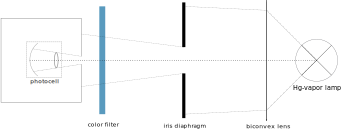
\includegraphics[width=.4\textwidth]{img/3-1-setup.pdf}
	\caption[Setup for measuring terminal voltage]{\textbf{Setup for measuring terminal voltage} The usage of a Hg-vapor lamp is necessary for sufficiently high photovoltages and -currents, as photons from the Hg-vapor lamp have higher energies than ambient photons.}
	\label{fig:term_volt}
\end{figure}
The setup in \autoref{fig:term_volt} is used to measure the terminal voltage of the photoelectric cell for different wavelengths.
Wavelengths are toggled through by placing different color filters in the beam path.
The used buffer amplifier is zeroed to allow for high precision measurements.
Varying $\lambda$, the voltage $U$ across the photoelectric cell is measured.

Conservation of energy yields
\begin{align}
	eU &= h\nu+E_\text{A} \nonumber \\
	\Leftrightarrow U &= \frac{hc}{e}\cdot\lambda^{-1}+\frac{E_\text{A}}{e}, \label{eq:energy_balance}
\end{align}
where $E_\text{A}$ denotes the activation energy of the photocathode material.
This equation can be used to compute the $\frac{h}{e}$-ratio.

\textbf{Evaluation}\\
\begin{figure}[tbp]
	\centering
	\includegraphics[width=.6\textwidth]{./data/plots/3-1.pdf}
	\caption[Linear regression of terminal voltage over inverse wavelength]{\textbf{Linear regression of terminal voltage over inverse wavelength} Three series of data points are averaged and a linear fit is applied. $a=\SI{922.7}{\volt\meter}$, $b=\SI{-985.3}{\milli\eV}$, $R^2=99.5\%$}
	\label{fig:}
\end{figure}
\section{Stopping Voltage}%3.2 and 3.5


\section{Photocurrent}%3.3 and 3.4

The current flowing through the photoelectric cell is measured while the voltage across its terminals is held at constant levels ranging from \SIrange{-3}{6}{\volt}.
The experiment is repeated with a neutral density filter in front of the mercury lamp.

\textbf{Setup}\\
A schematic of the setup is shown in \autoref{sch:photocurrent}.
A shunt resistor of $R_\text{shunt} = \SI{100}{\mega\ohm}$ is used, the output voltage $U_\text{out}$ is buffered by the electrometer to minimize the additional load.
The voltage $U_\text{g}$ is generated by a potentiometer connected across a \SI{9}{\volt} battery, it is read from a panel meter.

The actual stopping potential is $U_\text{s} = U_\text{g} - U_\text{out}$, the photocurrent is calculated as $I_\text{ph} = \frac{U_\text{out}}{R_\text{shunt}}$.

\textbf{Evaluation}\\
The measured values for the series with and without filter are plotted in \autoref{plt:photocurrent}.
There is no measurable reverse current, so measurements for $U_\text{g} < \SI{-1.6}{\volt}$ are omitted.

Both curves start around \SI{-1.5}{\volt} looking similar to the characteristic diode curve.
For higher stopping potentials, the current approaches the saturation current.

To approximate the saturation current, a logistic curve is fitted to the data as it is the most accurate model tested:
\begin{equation*}
	I_\text{ph}(U_\text{s}) = \frac{I_\text{sat}}{1 + \mathrm{e}^{-b (U_\text{s} - U_0)}},
\end{equation*}
resulting in
\begin{gather*}
	I_\text{sat} = \SI{37}{\nA}, \quad U_0 = \SI{1.64}{\volt}, \quad b = \SI{1.28}{\per\volt} \tag{no filter}\\
	I_\text{sat} = \SI{23}{\nA}, \quad U_0 = \SI{1.86}{\volt}, \quad b = \SI{1.15}{\per\volt}. \tag{filter}\\
\end{gather*}

The saturation current is proportional to the filter's transmittance, so the transmittance can be calculated as
\begin{equation*}
	T = \frac{I_\text{sat, filter}}{I_\text{sat, \#nofilter (todo)}} = \num{0.62}.
\end{equation*}

\begin{figure}[tbp]
	\centering
	\includegraphics[width=.4\textwidth]{img/photocurrent.pdf}
	\caption[Setup for measuring Photocurrent]{\textbf{Setup for measuring Photocurrent}}
	\label{sch:photocurrent}
\end{figure}

\begin{figure}[tbp]
	\centering
	\includegraphics[width=.8\textwidth]{data/plots/photocurrent.pdf}
	\caption[Photocurrent versus Stopping Potential]{\textbf{Photocurrent versus Stopping Potential}}
	\label{plt:photocurrent}
\end{figure}
